\documentclass[11pt]{article}
\usepackage{latexsym}
\usepackage{graphicx}
\usepackage{amsmath,amssymb,amsthm}
\usepackage{epsfig}
\usepackage[right=0.8in, top=1in, bottom=1.2in, left=0.8in]{geometry}
\usepackage{setspace}
\usepackage[utf8]{inputenc}
%\spacing{1.06}

\newcommand{\handout}[5]{
  \noindent
  \begin{center}
  \framebox{
    \vbox{\vspace{0.25cm}
      \hbox to 5.78in { {University of Wrocław:\hspace{0.12cm}Algorithms for
          Big Data (Fall'19)} \hfill #2 }
      \vspace{0.48cm}
      \hbox to 5.78in { {\Large \hfill #5  \hfill} }
      \vspace{0.42cm}
      \hbox to 5.78in { {#3 \hfill #4} }\vspace{0.25cm}
    }
  }
  \end{center}
  \vspace*{4mm}
}

\newcommand{\lecture}[4]{\handout{#1}{#2}{#3}{Scribe:\hspace{0.08cm}#4}{Lecture #1}}

\newtheorem{theorem}{Theorem}
\newtheorem{corollary}[theorem]{Corollary}
\newtheorem{lemma}[theorem]{Lemma}
\newtheorem{observation}[theorem]{Observation}
\newtheorem{example}[theorem]{Example}
\newtheorem{definition}[theorem]{Definition}
\newtheorem{claim}[theorem]{Claim}
\newtheorem{fact}[theorem]{Fact}
\newtheorem{property}[theorem]{Property}
\newtheorem{assumption}[theorem]{Assumption}

\newcommand{\E}{{\mathbb E}}
\DeclareMathOperator{\var}{Var}
\newcommand{\eps}{\varepsilon}
\newcommand{\bigo}{\mathcal{O}}
\setcounter{MaxMatrixCols}{20}

\begin{document}

\lecture{12: Coresets}{ 13/01/2020}{Lecturer: \emph{Przemysław Uznański }}{-}


\section{Coresets}
Setup: given set of $P \subseteq \mathbb{R}^d$, compute $C_P() : \mathbb{R}^d \to \mathbb{R}$. For example:
\begin{itemize}
\item $MEB$, a minimal enclosing ball: $C_P(o)$ is a radius of minimal enclosing ball for set $P$ centered at $o$. 
\end{itemize}

$|P| = n$ is large, so storing it explicitly is out of the question. Observe that for fixed $o$, a single $p \in P$ is enough, that is $\forall_o \exists_{p \in P} C_P(o) = C_{\{p\}}(o)$. Can we generalize this observation so it works for all $o \in \mathbb{R}^2$ at once?

\begin{definition}
We say that $S \subseteq P$ is a $c$-coreset for $P$ if for any $o$ and any $T \subseteq \mathbb{R}^d$ there is:
$$C_{S \cup T}(o) \le C_{P \cup T}(o) \le c \cdot C_{S \cup T}(o)$$
\end{definition}

Note: this is a stronger definition than just requiring that $f_{S}(o)$ is a $c$-approximation to $C_{P}(o)$ (take $T = \emptyset$).

Observe that in case of $MEB$ we have for $A \subseteq B$: $C_A(o) \le C_B(o)$, so the first inequality is ''for free''.

\begin{lemma}[Merge property]
If $S$ is a $c$-coreset for $P$, and $S'$ is a $c$-coreset for $P'$, then $S \cup S'$ is a $c^2$-coreset for $P \cup P'$.
\end{lemma}

\begin{lemma}[Reduce property]
If $S$ is a $c$-coreset for $P$ and $P$ is a $c$-coreset for $Q$, then $S$ is a $c^2$-coreset for $Q$.
\end{lemma}


We sometimes want a stronger property (which for example MEB satisfies)
\begin{property}[Disjoint merge]
If $S$ is a $c$-coreset for $P$ and $S'$ is a $c$-coreset for $P'$ and $P \cap P' = \emptyset$, then $S \cup S'$ is a $c$-coreset for $P \cup P'$.
\end{property}
Exercise: proof for MEB.

\begin{theorem}
Assume that a problem is supported by a $(1+\alpha)$-coreset of size $f(\alpha)$, computable in linear space, with disjoint merhe property. Then there is a streaming algorithm with $1+\varepsilon$ guarantee, with space $\bigo(f(\varepsilon/\log n) \log n)$.
\end{theorem}
\begin{proof}
Sketch of a proof: put stream of $n$ elements into binary tree. Each node stores coreset for the range below it. 

For two sibling nodes $N_1, N_2$ covering sets $A_1, A_2$, at level $i$, and parent node $N$ at level $i+1$, there is:
\begin{itemize}
\item $N_1$ is $(1+\alpha)^i$-coreset for $A_1$ (and the same for $N_2$, $A_2$)
\item $N_1 \cup N_2$ is $(1+\alpha)^i$-coreset for $A_1 \cup A_2$
\item $N$ is constructed as $(1+\alpha)$-coreset for $N_1 \cup N_2$
\item thuse $N$ is $(1+\alpha)^{i+1}$-coreset for $A_1 \cup A_2$
\end{itemize}

As a end-result, we have in the root $(1+\alpha)^{\log n}$-coreset for whole input. Selecting $\alpha = \bigo(\varepsilon/\log n)$ is enough.
\end{proof}

\subsection{Coreset for MEB}
Construction goes as follow. Choose dense set of directions $\{v_i\}_{i=1}^m$, such that for any other direction $u$, there is always some $v_i$ such that $\text{angle}(u,v_i) \le \alpha$: this is $\sim \alpha$-net on unit-ball (up to trigonometry). We can choose such set of $m = (1/\alpha)^{\bigo(d)}$ directions.

\begin{claim}
For any direction $v_i$, pick $p_i \in P$ that is extremal in that direction. 
Set $S = \{p_i\}_{i=1}^m$  is a $(1+\bigo(\alpha^2))$-coreset for $P$.
\end{claim}
\begin{proof}
Pick arbitrary $T$ ($T= \emptyset$ w.l.o.g. in this proof), and $P$ and constructed set $S$. Fix $o$. Pick furthest point $x \in P$, and close direction $v_i$, and maximal in this direction point $p_i \in S$. The angle $x$-$o$-$p_i$ is small (at most $\alpha$), so the stretch is upperbounded by $\frac{1}{\cos \alpha} = 1 + \bigo(\alpha^2)$.
\end{proof}

\subsection{Coreset for median}
Approximate median: given sequence of numbers $A$ of number $a_1,\ldots,a_n$, return $a$ such that $(1/2 \pm \varepsilon)n$ elements in $A$ are smaller/larger than $a$.

Alternative formulation: find $a$ that minimizes $C_A(a) = \max( |\{i : a_i \ge a\}|, |\{i : a_i \le a\}| )$.

Coreset of size $1/\varepsilon$: pick every $\varepsilon n$ element from sorted $A$.
Easy to see that
$$C_{A \cup T}(a) \le C_{A \cup S}(a) \le (1+\varepsilon) C_{A \cup T}(a)$$

Plugging into the theorem, we obtain streaming median computation in space $\bigo(\log^2 n / \varepsilon)$. In fact this works for any quantile computation (but the error is additive). Improvement: pre-filter and keep only $1/\varepsilon^2$ elements (randomly), so space becomes $\bigo(\log^2 (1/\varepsilon) / \varepsilon)$.

\section{Graph algorithms}
\subsection{Certificates}
Graph-theoretic approach, for decision problems.

\begin{definition}
For property $\mathcal{P}$, and a graph $G$, we say that $G'$ is a strong certificate for $G$ if: for any $H$, $G\cup H$ is in $\mathcal{P}$ iff $G' \cup H$ is in $\mathcal{P}$.
\end{definition}

Examples:
\begin{itemize}
\item connectivity: any spanning forest
\item non-bipartiteness: any spanning forest + single odd-cycle inducing edge
\item edge/vertex connectivity
\end{itemize}

\subsection{Spanners}

Subgraph approximately preserving distances:

\begin{definition}
$H$, an edge subgraph of $G$, is a $t$-spanner of $G$, if for any $u,v$ there is
$$d_H(u,v) \le t \cdot d_G(u,v)$$
\end{definition}

\begin{theorem}
Any unweighted $G$ contains $t$-spanner with $\bigo(n^{1+2/(t-1)})$ edges, and it can be computed in one pass.
\end{theorem}
\begin{proof}
Maintain subgraph. Process edges one-by-one. If an edge causes a cycle of length $\le t+1$, do not insert it.
\begin{enumerate}
\item This constructs a $t$-spanner. (Nice easy exercise) \\

\begin{proof}
	 Let's denote a spanner by $H$ as previously. \\
	\begin{itemize}
		\item (by contradiction) Assume that $H$ maintained in that way is not a \textit{t}-spanner. So, there exist a pair of vertices $u,v$ (counterexample) s.t. $d_H(u,v) > t d_G(u,v)$. Let's choose some shortest path between $u,v$ in G, $P_G$ and in $H$, $P_H$. The proof will have three stages. 
		\begin{center}
			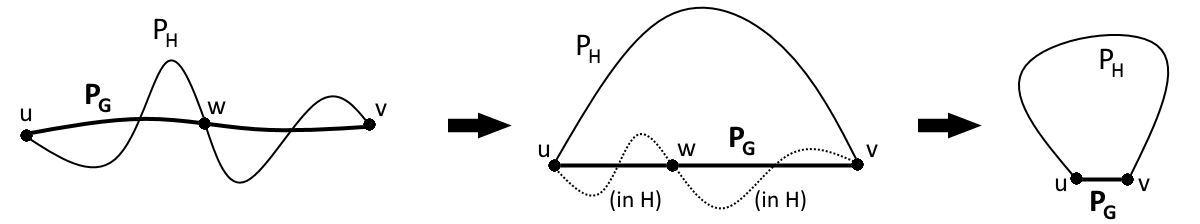
\includegraphics[width=\linewidth]{lecture_12_proof_stages.png}
		\end{center}
		\item Now we argument that there also exists a counterexample s.t. $P_G$ and $P_H$ don't cross - only common vertices between them are $u, v$. This follows, because if there is a vertex $w$ s.t. $w \neq u, w \neq v, w \in P_G, w \in P_H$, then we can substitute one of $u, v$ (wlog, $u$) with $w$ in the counterexample. That's because $P_G, P_H$ are shortest paths between $u,v$ in $G,H$, so the equalities below are true (if they wouldn't be, there would exist some shorter path):
		$$ d_H(u,w) + d_H(w,v) = d_H(u,v) > td_G(u,v) = td_G(u,w) + td_G(w,v)$$
		so either $d_H(u,w) > td_G(u,w)$ or $d_H(w,v) > td_G(w,v)$ (in other case contradiction by summing sides of opposite ($\leq$) inequalities). By substituting $u \leftarrow w$ as many times as needed we have $P_G \cap P_H = \{u,v\} $.
		\item We have that $P_G, P_H$ only have $u,v$ common and now we argument that there also exists a counterexample s.t. $|P_G|=1$. Similarly as previously, if there exists some $w$ on $P_G$ between $u,v$, we can substitute one of $u,v$ (wlog, $u$) with it in the counterexample. This is because from triangle inequality in $H$ we have (please note that there is no longer an equality in the left part because $w$ is not on $P_H$ and we need paths for $d_H(u,w), d_H(w, v)$ that contain some edges from outside of $P_H$, but the equality in the right part which we need is still true as $w \in P_G$):
		$$ d_H(u,w) + d_H(w, v) \geq d_H(u,v) > td_G(u,v) = td_G(u,w) + td_G(w,v)$$
		then by same argument as previously, either $d_H(u,w) > td_G(u,w)$ or $d_H(w,v) > td_G(w,v)$. By substituting $u \leftarrow w$ as many times as needed, we finally have that $u,v$ are neighbours in $G$ (please note that by such substitution, we can again have intersections between $P_G, P_H$ and we may need to move to the previous step, but $|P_G|$ constantly decreases).
		\item As we now have a counterexample where $|P_G|=1$ and $|P_H|>t|P_G|=t$, we arrive at a contradiction: when we were processing the only edge on $P_G$, we should have added it to $H$ as it didn't cause a cycle of length $\leq t+1$ - it doesn't cause that now as $d_H(u,v) = |P_H| \geq t+1$ and in the time of processing of that edge it also didn't as $H$ at that time was a subgraph of the final $H$.
	\end{itemize}
\end{proof}
\item The graph is sparse enough:
\begin{itemize}
\item Let $d = 2m/n$ be average degree.
\item There is subgraph $H$ of $G$ with minimum degree $d' = d/2$: keep removing vertices with degree smaller than $d'$. We cannot end with no vertices, since then we removed less than $m$ edges.
\item $H$ has every vertex of degree at least $m/n$, and no cycle of length $t+1$ or less.
\item BFS tree of depth $t/2$ has no cycles in $H$
\item $(m/n-1)^{t/2} \le |H| \le n$, which implies bound on $m$
\end{itemize}
\end{enumerate}
\end{proof}


\end{document}


